\chapter{Background} \label{background}

\section{Blockchain}
Pre-processing plays an important role in image detection. The aim of pre-processing is improving the construct the raw image and enhancing features of the image which is appropriate in further processing.

% \subsection{Grayscale image}
% For flowchart, color is not a important feature to keep in recognition procedure and color also causes the detection algorithm more complex. Therefore, we need to remove this feature by converting the image into grayscale image. In this part, we represent some fundamental method to convert a RGB image into grayscale image.
% \begin{itemize}
%     \item Average method is the most simple one, we only need to take the average of three colors red, green and blue ($(R+G+B)/3$)
%     \item Lightness method averages the most prominent and least prominent colors ($(max(R, G, B) + min(R, G, B)) / 2$)
%     \item Luminosity method forms a weighted average to account for human perception. Human are more sensitive to green than other colors, so green is weighted most heavily ($0.299 R + 0.587 G + 0.114 B$)
% \end{itemize}

% \subsection{Histogram equalization}
% Histogram equalization is a technique used to improve contrast in image by spreading out the most frequent intensity values. By accomplishing this, histogram equalization allows the image’s areas with lower contrast to gain a higher contrast. This technique includes steps as below:
% \begin{itemize}
%     \item Calculate the histogram $H(i)$ of the image by counting the total number of pixels which has similar intensity value.
%     \item Calculate the cumulative distribution $H'(i)$ from $H(i)$ with the formula: $H'(i) = \sum \limits_{j=0}^i  H(j)$
%     \item Normalize $H'(i)$ such that the maximum value equals the maximum value for the intensity of the image which is 255
%     \item Mapping lightness values with $H'(i)$ to obtain the equalized image with the formula: \\ $equalizedImage(x,y) = H'(srcImage(x,y))$
% \end{itemize}
% \subsection{Noise filtering}
% As we introduce about noise in the Chapter \ref{introduction}, noise filtering techniques plays an important role in the pre-processing procedure. In this part, we give some fundamental approaches such as Gaussian filter which is simple and suitable for Gaussian noise and Median filter which is better than Gaussian filter in preserving edges according to \cite{56}. In the Chapter \ref{chap:exp}, we are going to compare these two approaches with a captured image in our project.

% \subsection{Binarization}
% Image binarization is the process of converting a grayscale image to a black-and-white image, essentially reducing the information contained within the image from 256 shades of gray to 2 which are only black and white. The approach used in this part is Adaptive Thresholding. In simple thresholding, the threshold value is global for all the pixel in image, while Adaptive thresholding is the method where the threshold value is calculated for smaller regions and therefore, there will be different threshold values for different regions. Therefore, this approach gives a better result than simple thresholding.

\section{HDWallet}
We decided that there would be two algorithms in our project. One detection will be faster and one will be more accurate. For the Two Stages Detection, we are planning to use Faster R-CNN with RPN and RoI Align. For the One Stage Detection, we are trying to use both YOLO v4 and RefineDet and select whichever yield better result.
\subsection{Category}
As introduced in earlier section, Faster R-CNN extends Fast R-CNN by introducing Region Proposal Network
A Faster R-CNN consists of three parameters: Backbone CNN, RPN and Classification model.
% \subsubsection{Backbone CNN}
%     The Convolutional Neural Network is an important part in the algorithm. The better the CNN is, the higher accuracy the model will have. Currently, we are making an experiment on three different network: ResNet50, Inception v4 and Inception ResNet v2. The reason we decide to do so is because ResNet50 is a lightweight model and Inception v4/Inception ResNet v2 provides higher results with computational tradeoff according to \href{https://github.com/alyato/CNN-models-comparison}{this page}.
% \begin{figure}[!t]
%     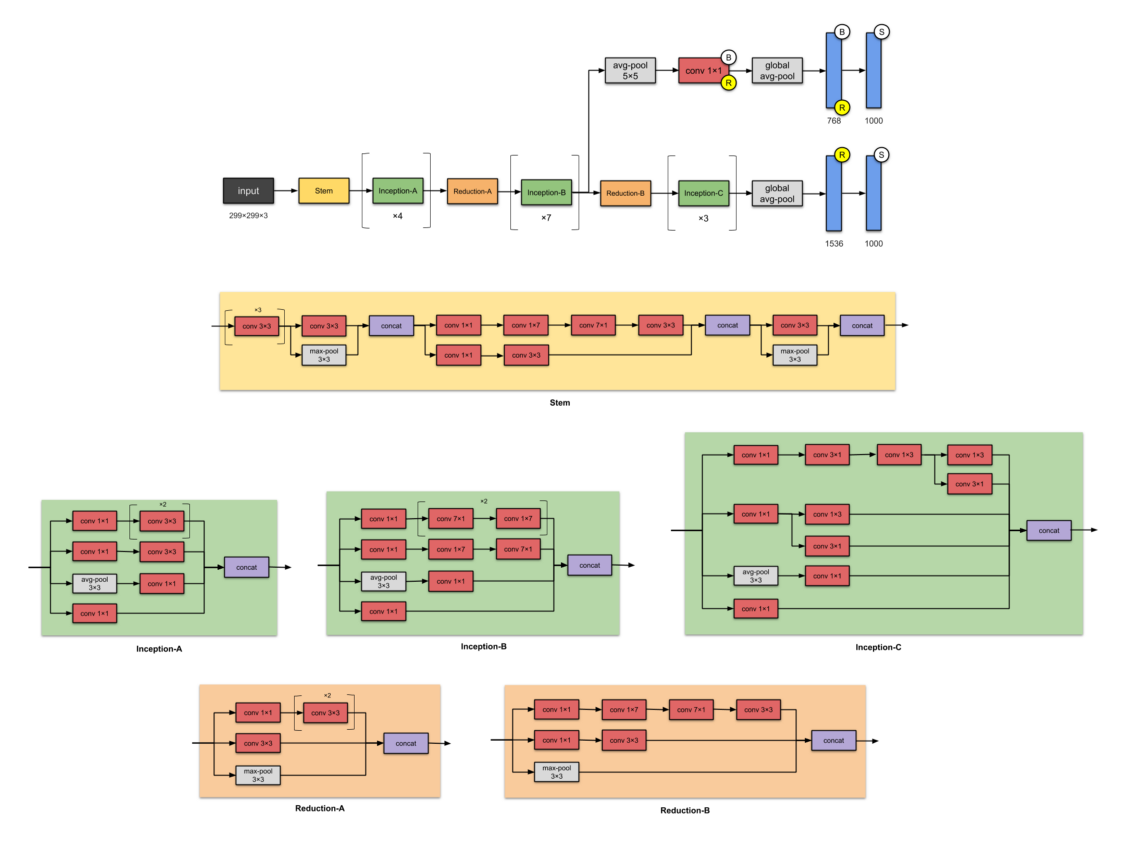
\includegraphics[width=14cm]{Images/recognition/Inception_v4.png}
%     \caption{Inception v4 model}
%     \label{fig: Inception v4}
% \end{figure}
\subsection{Coins}

\subsection{Wallet structure}

\section{Cryptography}

\subsection{Cryptographic hash}

\subsection{Diffie-Hellman algorithm}

\subsection{RSA}

\subsection{ECC}

\subsubsection{Blockchain: secp256k1}

\subsubsection{Discrete logarithm problem}

\subsection{Twisted-Edward curve and Ed25519}

\subsection{Key derivation function}



% \subsubsection{Regional Proposal Network}

%     RPN is a small network that slides over a convolutional feature map which is the output by the last convolution layer. It has a classifier and a regressor. In the first step, the input image goes through a CNN to give the  output as a set of feature maps on the last layer. Next, a sliding window is run spatially on these feature maps. For each sliding window, a set of 9 anchors are generated which all have the same center but with 3 different aspect ratios and 3 different scales. Furthermore, for each of these anchors, a value p* is computed which indicated how much these anchors overlap with the ground-truth bounding boxes. p* is calculated by:
%     \[
%     p^* =
%     \begin{cases}
%         1       & \text{if } k\ge 0.7\\
%         -1,      & \text{if } k\le 0.3\\
%         0       & \text{otherwise}
%     \end{cases}
%     \text{where} k = \frac{\text{Anchor} \cap \text{GroundTruthBox}}{\text{Anchor} \cup \text{GroundTruthBox}}
%     \]
    
%     Lastly, The 3×3 spatial features extracted are fed to classification and regression. The output of regressor is the predicted bounding box, the output of classifier is the probability that the box contain an object or background. 
% \begin{equation}
%     \begin{aligned}
%     t &= [(x - x_a)/w_a, (y - y_a)/h_a, log(w/w_a), log(h/h_a)]\\
%     t^* &= [(x^* - x_a)/w_a, (y^* - y_a)/h_a, log(w^*/w_a), log(h^*/h_a)]\\
%     \text{Loss function:} L({p_i}, {t_i}) &= (1/N_{cls}) L_{cls}(p_i,p_i^*) + \lambda (1/N_{reg}) L_{reg}(t_i,t_i^*)
%     \end{aligned}
% \end{equation}
        
    
%     p* with regression term in the loss function ensures that if and only if object is identified as yes, then only regression will count, otherwise p* will be zero, so the regression term will become zero in the loss function.
    
% \subsection{Feature Pyramid Network}
% Feature pyramids is a component in recognition systems for detecting objects at different scales. It consists of two main components:

% \begin{itemize}
%     \item Bottom-up Pathway: The bottom-up pathway is the feed-forward computation of the backbone CNN. It is defined that one pyramid level is for each stage. The output of the last layer of each stage will be used as the reference set of feature maps for enriching the top-down pathway by lateral connection. Normally, one layer has its size equal to 1/2 of the previous layer.
%     \item Top-down Pathway and Lateral Connection: The feature map at the highest layer in the bottom-up pathway is brought to the corresponding one of the Top-down pathway. For every layer under it, a lateral connection is constructed by the following steps: The upper layer is up by a factor of 2. The corresponding feature map from bottom-up is undergone through a 1x1 convolution to reduce dimension. Finally, both feature maps from bottom up and top down are merged by element-wise addition.
%     After the final layer is computed, or the algorithm stop when reaching a certain level, all merged layers go through a 3x3 Convolution layer to generate the final feature map.
% \end{itemize}
% \begin{figure}[!t]
%     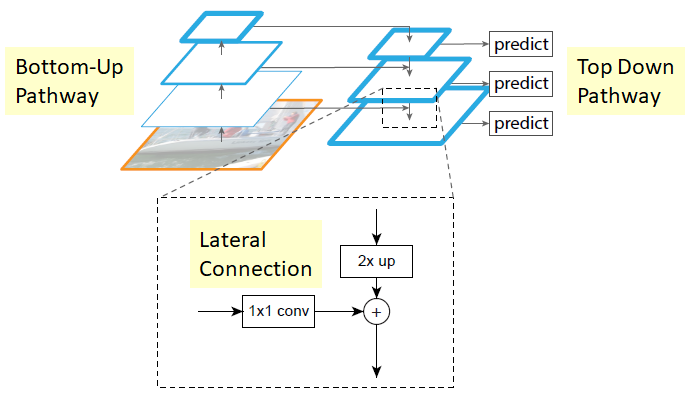
\includegraphics[width=14cm]{Images/recognition/FPN.png}
%     \caption{Feature Pyramid Network}
%     \label{fig: FPN}
% \end{figure}


% \subsection{Region of Interest Align}
% Mask R-CNN introduces a new algorithm called Region of Interest Align. It replaces the RoI Pooling in Faster R-CNN. RoI Align deals with the round-off errors that RoI Pooling cannot. 
% The difference was to introduce bi-linear interpolation when calculate the pixel’s value for the floating point coordinate. For example (69.5, 420.7). This is a floating point coordinate. We however know the what pixel value for (69, 420) and (70, 421). So to estimate (69.5, 420.7) we can use a technique used in many image processing tricks that is called bi-linear interpolation.
% The step are processed as follow:
% \begin{itemize}
% \item The RoI pooling layer divide the feature map into M by N grid. For each small grid, the unit is then sampled K times. For the Mask R-CNN paper they used K=4 for best result.
% \item Divide each unit equally by 4 means finding the center pixel values for the these 4 regions in the unit. Of course these centers are floating point based. Therefore we use bi-linear interpolation to predict its value.
% \item After bi-linear interpolation, we perform max pooling on these 4 samples to output the unit’s value.
% \end{itemize}

% \begin{figure}[!t]
% \centering
% 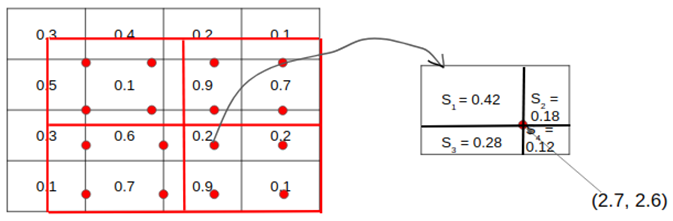
\includegraphics[width=14cm]{Images/recognition/RoI_Align.png}
% \caption{Region of Interest Align}
% \end{figure}

% \subsection{YOLO}
% \subsubsection{YOLO v1}
% \begin{figure}[!b]
% \centering
% 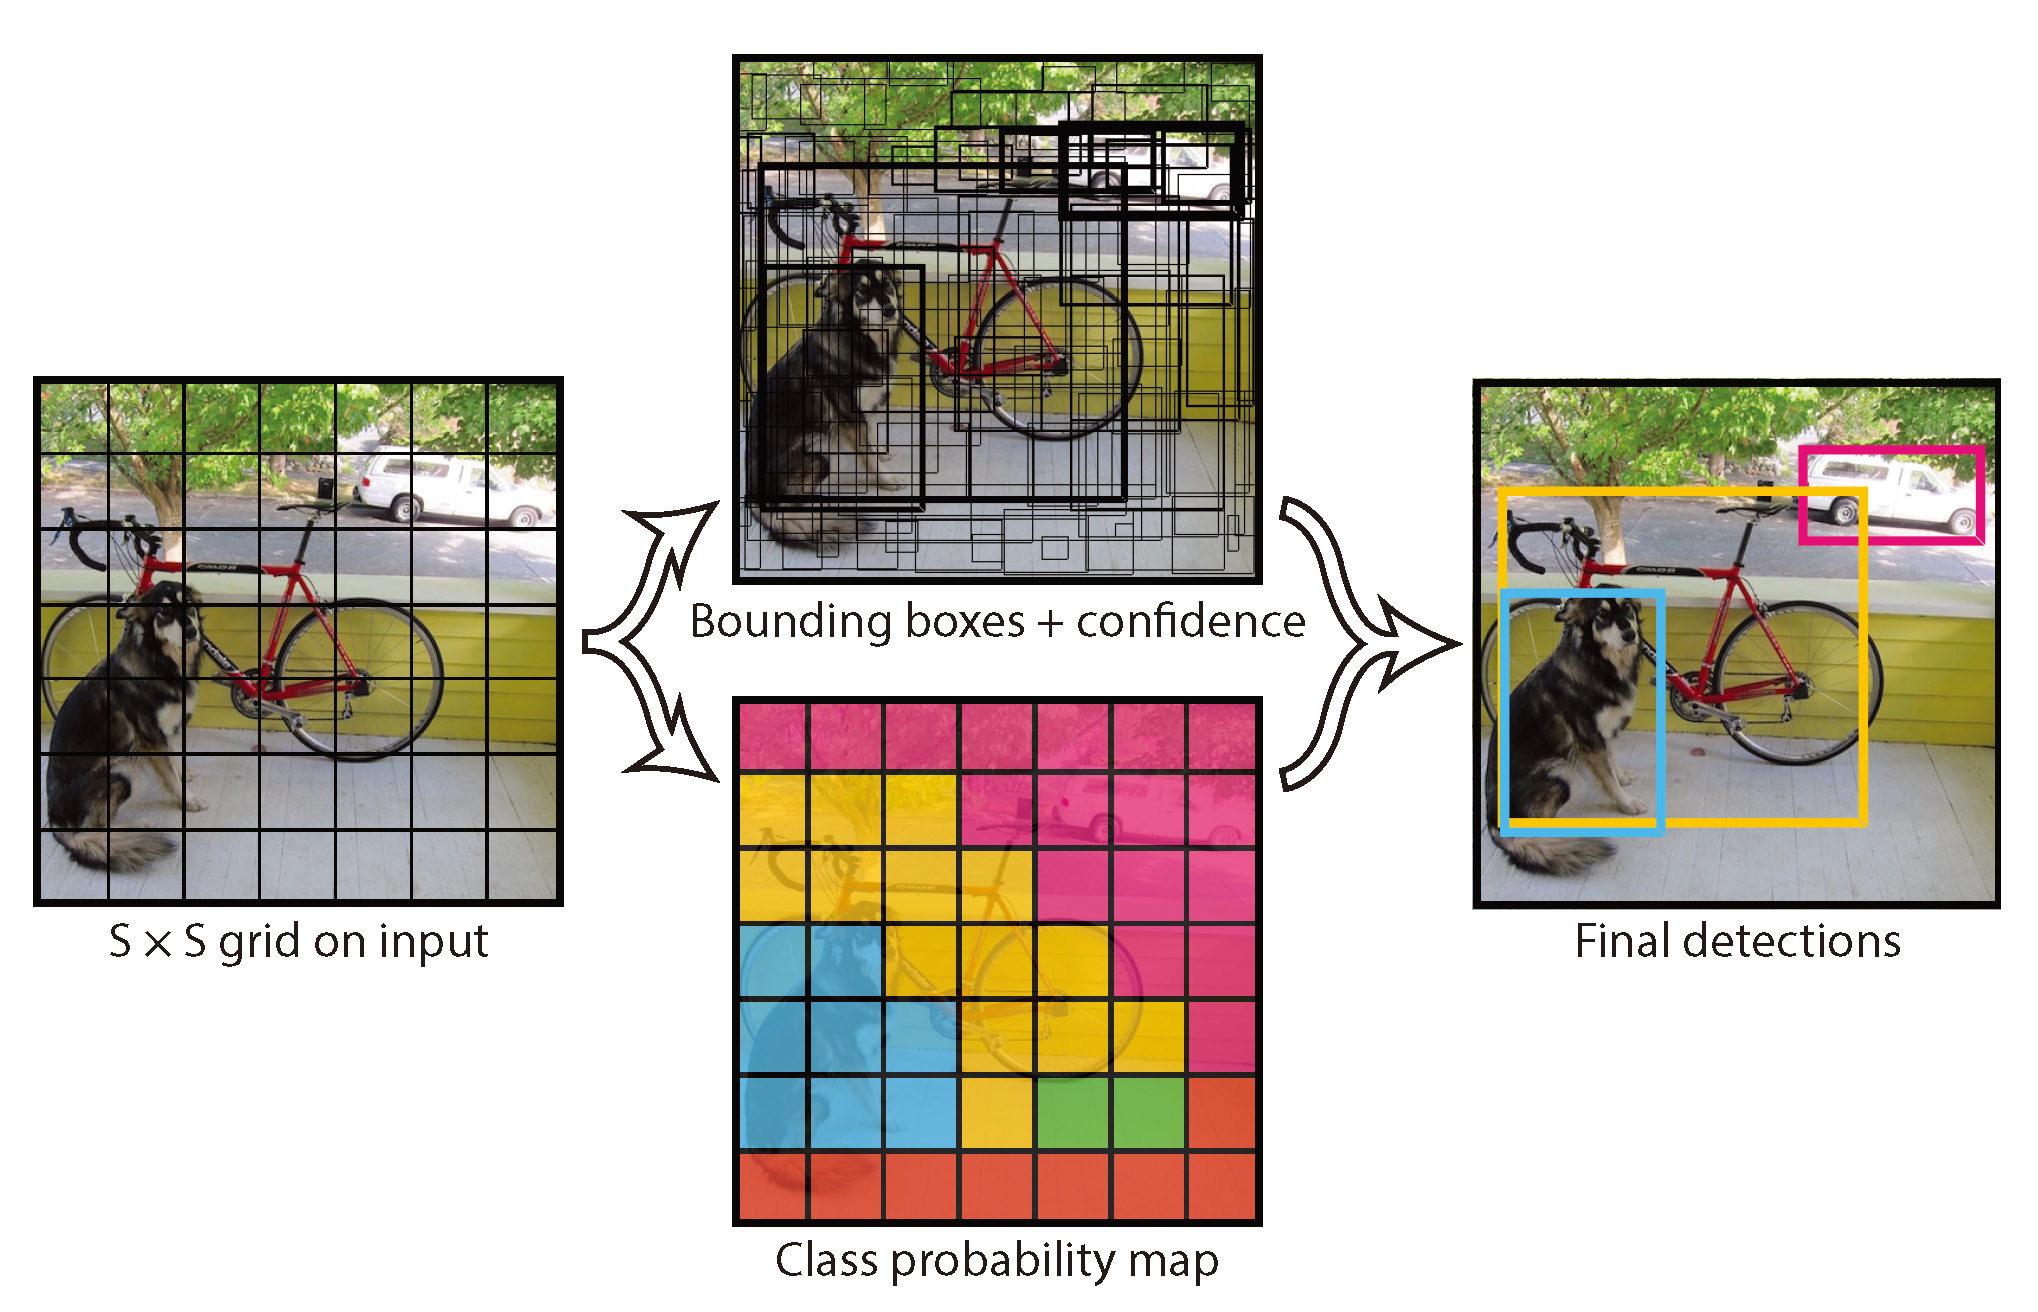
\includegraphics[width=14cm]{Images/recognition/YOLO.png}
% \caption{YOLO model}
% \label{fig: YOLO model}
% \end{figure}
% As figure \ref{fig: YOLO model} YOLO divides the input image into an S × S grid. For each object that is present on the image, one grid cell is said to be “responsible” for predicting it. That is the cell where the center of the object falls into. 

% Each grid cell predicts B bounding boxes as well as C class probabilities. The bounding box prediction has 5 components: (x, y, w, h, confidence). The (x, y) coordinates represent the center of the box, relative to the grid cell location. These coordinates are normalized to fall between 0 and 1. The (w, h) box dimensions are also normalized to [0, 1], relative to the image size. Confidence scores are calculated as Pr(Object) multiply with $IOU_{pred}^{truth}$.

% At the same time, regardless of the number of boxes, C conditional class probabilities (Pr(Class(i)|Object)) should also be predicted in
% each grid cell. It should be noticed that only the contribution from the grid cell containing an object is calculated. 
% At test time, class-specific confidence scores for each box are achieved by multiplying the individual box confidence predictions with the conditional class probabilities as:
% \begin{center}
%     $Pr(Object) * IOU_{pred}^{truth} * Pr(Class_i|Object) = Pr(Class_i) *IOU_{pred}^{truth}$
% \end{center}
% During training, the following loss function is considered as figure \ref{fig: YOLO_lost}
% \begin{figure}[!t]
% \centering
% 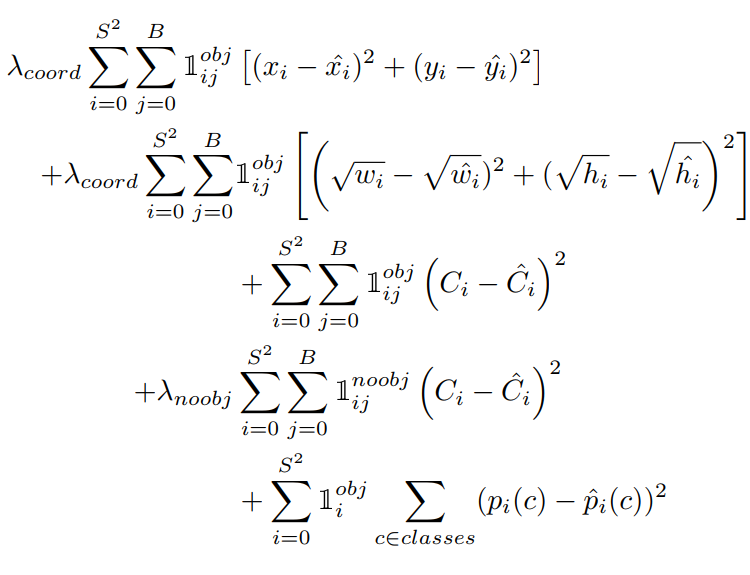
\includegraphics[width=14cm]{Images/recognition/YOLO_lost.png}
% \caption{Lost function of YOLO v1}
% \label{fig: YOLO lost}
% \end{figure}

% \subsubsection{YOLO v4}
% \begin{figure}[!t]
% \centering
% 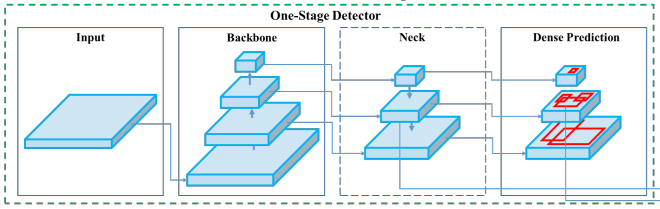
\includegraphics[width=14cm]{Images/recognition/YOLO_v4.png}
% \caption{YOLO v4}
% \label{fig: YOLO v4}
% \end{figure}

% YOLO v4 is the latest entry in this type of detector. YOLO v4 achieves really high accuracy with high speed. To get these results, YOLO v4 combines multiple features such as Weighted-Residual-Connections (WRC), Cross-Stage-Partial-connections (CSP), Cross mini-Batch Normalization (CmBN), Self-adversarial-training (SAT) and Mish-activation, Mosaic data augmentation, DropBlock regularization, and CIoU loss. 
% YOLO v4 consists of three main stages. The Backbone is a CNN model like ResNet, VGG are trained and tuned on detection dataset. THe neck is many extra layers that go in between the backbone and head. They are used to extract different feature maps of different stages of the backbone. The neck layer can be either FPN or Bi-FPN, which will be discussed on RefineDet. The head is a network doing the detection (classification and regression) of bounding boxes.

% \subsection{RefineDet}
% RefineDet is another candidate for us to use or improve in this project. From the previous chapter, we know that RefineDet is formed by two inter-connected modules: Anchor Refinement Module (ARM) and Object Detection Module (ORM). The system has three main element:
% \begin{itemize}
%     \item Transfer Connection Block is responsible for converting features of different layers from the ARM into the form required by the ODM, making ODM able to share features from ARM. Another function of the TCBs is to integrate large-scale context by adding the high-level features to the transferred features to improve detection accuracy. 
%     \item Two-Step Cascaded Regression: Most current method relies on one-step regression based on multiple feature layers. RefineDet is not the same, it uses a Two-Step Cascaded Regression strategy to regress the locations and sizes of objects.
%     \item Negative Anchor Filtering: In training phase, for a refined anchor box, if its negative confidence is larger than a preset threshold $\theta$ (i.e., set $\theta$ = 0:99 empirically), that box will be discarded. This helps refined hard negative anchor boxes and refined positive anchor boxes to train the ODM. In the inference phase, if a refined anchor box is assigned with a negative confidence larger than $\theta$, it will be discarded in the ODM for detection.
% \end{itemize}


